\chapter{Introduction}

Elementary particle physics aims to describe nature at its most fundamental level.
This thesis presents analyses of data obtained from high energy proton collisions, which search for evidence for or against new theoretical models of elementary particle physics.
This section introduces the theoretical context of these searches, describing first the theoretical model presently serving as the null hypothesis of elementary particle physics, then a few issues identified with this model, and finally some proposed solutions for these issues.

\section{The Standard Model of Particle Physics} \label{sec:standardmodel}

Modern elementary particle physics finds itself in a peculiar state.
Physicists have constructed a theoretical model, now called the Standard Model of Particle Physics (the Standard Model; SM), that is the most quantitatively accurate scientific model of any kind, consistent with experiment in almost every laboratory test, even when experimental uncertainty is smaller than a part per ten billion \cite{electronmu_exp,electronmu_th}, with its most famously accuract prediction displayed in Table~\ref{tab:electronmu}.
\begin{table}
\centering
\begin{tabular}{r l}
\multicolumn{2}{c}{$\mu_e$} \\
\hline
Experiment & 2.00231930436 (56) \\
Theory & 2.002319304363 (15)
\end{tabular}
\caption[Comparison of theoretical prediction and experimental measurement of the electron magnetic moment.]
        {A comparison of the leading experimental measurement of the electron's magnetic moment \cite{electronmu_exp}, and the Standard Model's theoretical prediction \cite{electronmu_th}, in terms of the classical prediction, the Bohr magneton. 
          Famously, this is the most accurate verification of theory by experiment in all of science. 
          The numbers in parentheses are the uncertainties, on the same order as the last digits printed.}
\label{tab:electronmu}
\end{table}

It is important to take this time to reflect on the Standard Model's astonishing accuracy, because the Standard Model is known with certainty to be imperfect, for a few reasons. 
A subset are discussed in Section~\ref{sec:SMproblems}.
Particle physicists have a theory {\it known} to be incomplete, only an approximation, and yet so accurate an approximation that no evidence in favor of any specific proposed extension has ever been found.
Modern particle physicists hope to find experimental clues by testing the Standard Model using any available means, including by comparing its predictions for the outcomes of high energy proton collisions with experimental data.

  \subsection{A Brief Description} \label{sec:SMdescription}

  The Standard Model is based in quantum field theory (QFT), which provides the general toolkit used to make calculations, and identifies the observed elementary particles as excitations of these underlying fields.
  Since every elementary particle corresponds directly to an underying field and vice-versa, for example ``the electron particle'' and ``the electron field'' are colloquially treated as synonyms.

  The SM itself, like every model of elementary particle physics based in QFT, consists of a list of particles present in nature and a description of their interactions with each other.
  The particles can be grouped in several ways, but by far the most significant is to group bosons and fermions.

  The bosons of the Standard Model are the photon (typically indicated by $\gamma$), the W$^+$ and W$^-$, the Z, the eight gluons, and the Higgs.
  Of these, the Higgs has no intrinsic angular momentum (``spin-0'') and the others have intrinsic angular momentum of exactly $\hbar$ (``spin-1'').
  One of the major insights obtained from QFT is that the existence of spin-1 particles requires the existence of fermions that interact with them, and vice versa.
  A fermion that interacts with a boson is said to be ``charged under'' the boson.
  Moreover, pure fermion interactions are forbidden, so that fermion-fermion interactions require a ``mediating'' boson under which both fermions are charged, while boson-boson interactions are perfectly acceptable
  For this reason, bosons are said to mediate fundamental interactions.
  The photon mediates electromagnetism, and the gluons collectively mediate the strong interaction, as described by quantum chromodynamics (QCD).
  For historical reasons, the distinct interactions mediated by the W$^+$ and W$^-$, the Z, and the Higgs are all collectively called the weak interaction.
  The bosons of the Standard Model are summarized in Table~\ref{tab:bosons}.

  \begin{table}
    \centering
    \begin{tabular}{r r l}
      Boson             & Mass (GeV) \cite{pdg} & Interaction \\
      \hline
      Photon ($\gamma$) & 0                     & Electromagnetism \\
      Gluon (g)         & 0                     & Strong (QCD) \\
      W$^{\pm}$         & 80.379 $\pm$ 0.012    & Weak (charged current) \\
      Z                 & 91.1876 $\pm$ 0.0021  & Weak (neutral current) \\
      Higgs (h)         & 125.18 $\pm$ 0.16     & Weak (symmetry breaking and mass) \\
    \end{tabular}
    \caption[Table of Standard Model bosons.]
            {The Standard Model bosons, their masses, and associated interactions. Note that there are eight gluons, but they are not experimentally distinct.}
            \label{tab:bosons}
  \end{table}

  The interactions have very different character due to differences in the mediating bosons.
  The photon and electromagnetism are most familiar.
  Electromagnetism is relatively simple, as a result of having only a single-component charge and a single mediating boson, and is relatively easily studied due to its long range, as a consequence of the masslessness of the photon.
  The weak interaction, by contrast, is less well-known in part due to its very short range, a consequence of the {\it large} masses of the mediating bosons.
  In addition to the $1/r^2$ behavior familiar from electromagnetism, forces are also suppressed by an exponential term, $e^{-\frac{mc^2}{\hbar c}r}$, where $m$ is the mass of the mediating boson and $\hbar c \approx 200$~GeV-pm.
  This term vanishes for massless bosons like the photon, but since the weak bosons have masses on the order of 100~GeV, the weak interaction becomes negligible after only a few picometers despite having an intrinsic interaction strength comparable to electromagnetism.
  Thus, the weak interaction has an impact only on nuclear and elementary particle physics.
  The strong interaction is also short ranged, with effects becoming significant only on the order of femtometers, but for an entirely different reason.
  As its name suggests, it is also intrinsically stronger than the other interactions.
  It will be discussed in Section~\ref{sec:hadronization}.

  The fermions of the Standard Model are all spin-$\frac{1}{2}$, and come in two major groups.
  The leptons are those fermions which do not participate in the strong interaction, and the quarks are those that do.
  The leptons can be further subdivided into the electrically charged leptons, like the electron, and the electrically neutral neutrinos, which having neither strong nor electromagnetic interactions can interact only weakly, and are ghostlike particles as a result.
  The quarks can be further subdivided into the up-type quarks, which are positively charged, and the down-type quarks, which are negatively charged.
  There are three of each quark, one for each of the charges of the strong interaction, but like the eight gluons, they are not experimentally distinct.

  As is evident in Table~\ref{tab:fermions}, the fermions of the Standard Model occur in triplets with identical properties aside from mass: the up-type quarks, the down-type quarks, the charged leptons, and the neutrinos are all roughly three versions of the same particle with different masses.
  The fermions are said to be arranged in three roughly equivalent generations, with generation 1 having the least mass and generation 3 the greatest.

  \renewcommand{\arraystretch}{1.2}
  \begin{table}
    \centering
    \begin{tabular}{l c r r}
      Fermion             & Symbol & Mass (GeV) \cite{pdg} & Electric charge \\
      \hline
      Up quark            & $u$    & $0.0022^{+0.0005}_{-0.0004}$      & +$\frac{2}{3}$  \\
      Charm quark         & $c$    & $1.275^{+0.025}_{-0.035}$       & +$\frac{2}{3}$  \\
      Top quark           & $t$    & $173.0 \pm 0.4$       & +$\frac{2}{3}$  \\
      Down quark$^*$      & $d$    & $0.0047^{+0.0005}_{-0.0003}$      & -$\frac{1}{3}$  \\
      Strange quark       & $s$    & $0.095^{+0.009}_{-0.003}$       & -$\frac{1}{3}$  \\
      Bottom quark        & $b$    & $4.18^{+0.04}_{-0.03}$       & -$\frac{1}{3}$  \\
      \hline
      Electron            & $e$    & $0.0005109989461$(31) & $-1$ \\
      Muon                & $\mu$    & $0.1056583745$(24)  & $-1$ \\
      Tau                 & $\tau$    & $1.77686$(12)  & $-1$ \\
      Neutrinos           & $\nu_{e}$, $\nu_{\mu}$, $\nu_{\tau}$ & 0$^{\dagger}$ & 0 \\
    \end{tabular}
    \caption[Table of Standard Model fermions.]
    {A table of the Standard Model fermions, first the quarks then the leptons.
      The vastly different experimental character of quarks due to their confinement by the strong interactions make their masses much more difficult to measure than those of the charged leptons.
      Note that every Standard Model fermion also has an antiparticle, with identical properties except for opposite charge.
      (*) The charge and mass eigenstates of (by convention) down-type quarks are different, so that for example ``the mass of the down quark'' does not exist. Otherwise, decays across generations would be impossible. In practice, they are so nearly equal that the mass of the down quark is equated with that of the lightest mass eigenstate, etc.
      ($\dagger$) The Standard Model predicts that neutrinos are massless but they experimentally have nonzero masses, albeit one million times smaller than the electron's, see Section~\ref{sec:SMproblems}.
}
            \label{tab:fermions}
  \end{table}
  \renewcommand{\arraystretch}{1}

  If each generation were truly independent of the others, then each would be independently stable, as there would be no way to cross from, say, generation 3 to generation 1.
  However, it is an experimental fact that quarks can decay across generations via their interactions with the W boson, albeit much more slowly than within generations.
  This is well-accomodated in the Standard Model \cite{cabibbo,ckm}, in which there is no reason in general for the charge eigenstates with respect to any given boson to be equal to those of any other.
  The Higgs interaction eigenstates, being the mass eigenstates, are priviliged as the only charge eigenstates that are also eigenstates of the Hamiltonian, and so are the only states that can actually be produced.
  The hybrid nature of the physical states with respect to W interactions produces effective generation-crossing interactions for quarks described by the Cabibbo-Kobayashi-Maskawa (CKM) matrix, with values measured experimentally to be approximately \cite{pdg},
  \begin{equation} \label{eqn:ckm}
    \begin{bmatrix} 
      |V_{ud}| & |V_{us}| & |V_{ub}| \\
      |V_{cd}| & |V_{cs}| & |V_{cb}| \\
      |V_{td}| & |V_{ts}| & |V_{tb}| 
    \end{bmatrix}
\approx
    \begin{bmatrix} 
      0.974 & 0.224 & 0.004 \\
      0.218 & 0.997 & 0.042 \\
      0.008 & 0.039 & 1.019
    \end{bmatrix}
  \end{equation}
  where $V_{xy}$ indicates the effective coupling between quarks $x$ and $y$.
  If the eigenstates were exactly equal, the CKM matrix would be diagonal, with $V_{xx} = 1$ and $V_{xy} = 0$ ($x \neq y$), prohibiting trans-generation decays.
  As can be seen in Equation~\ref{eqn:ckm}, the CKM matrix is {\it nearly} diagonal, meaning trans-generation decays are slow but not impossible.
  This causes the bottom quark to have a longer lifetime than the charm quark despite having a larger mass, because a bottom quark must cross a generation to decay using $|V_{ub}| \approx 0.004$ or $|V_{cb}| \approx 0.042$ (the top quark is more massive), while a charm quark does not and may decay using $|V_{cs}| \approx 0.997$ (the strange is less massive).
  In fact, the bottom quark lifetime is long enough to be macroscopic, producing decay lengths on the order of millimeters.
  This is experimentally relevant, as discussed in Section~\ref{sec:btagging}.
  Similar physics is possible for leptons since neutrinos are now known to be massive, but is not incorporated in the Standard Model, in which neutrinos are massless, see Section~\ref{sec:SMproblems}.

  The detailed interactions of the Standard Model are more conveniently discussed using Feynman Diagrams, in the next section.

  \subsection{Feynman Diagrams and Perturbative Expansions} \label{sec:feyndiags}

  The interactions of the Standard Model are expressed as a Langrangian density, of intimidating complexity.
  Applying the Euler-Lagrange equations to this Lagrangian produces nonlinear differential equations that have no known exact solutions.
  However, it is possible to extract an approximate solution as a perturbative expansion in powers of the coupling, a parameter that indicates the intrinsic strength of an interaction.
  This procedure at first seems barely feasible, as it is no trivial task to find all the contributions to the leading order term, then the next to leading order term, and so on by simple inspection of the Lagrangian.
  Fortunately, physicist Richard Feynman was able to devise a diagrammatic method for expressing the terms of the perturbative expansion that is far more intuitive.

  First, once may inspect each term of the Lagrangian to assemble so-called vertices, the building blocks of diagrams.
  Each field that occurs in a term represents one line, and all the lines of a term intersect at a central point to form the vertex.
  For example, the Standard Model Lagrangian contains a term in which the electron field appears twice and the photon field appears once, from which one obtains the vertex shown in Figure~\ref{fig:eegamma}.
  Each vertex represents one power of the coupling.
  The diagrams with the fewest vertices, then, are the lowest order diagrams in the perturbative expansion.

  \begin{figure}[h!]
    \centering
    \begin{fmffile}{eegamma}
      \begin{fmfgraph*}(40,25)
        \fmfleft{i1,i2}
        \fmfright{o1,o2}
        \fmfbottom{b}
        \fmf{fermion,label=$e^-$,label.side=left}{i2,v1}
        \fmf{fermion,label=$e^-$,label.side=left}{v1,o2}
        \fmf{photon,label=$\gamma$,label.side=left}{v1,b}
      \end{fmfgraph*}
    \end{fmffile}

    \caption[The fundamental vertex of electromagnetism.]{
      The Standard Model Lagrangian contains a term in which the electron field appears twice, and the photon field once, which corresponds to this Feynman diagram vertex.
      This vertex, and analogous vertices in which another fermion replaces the electron, are the vertices of electromagnetism.      
      Traditionally, straight lines with arrows represent fermions, and a wavy line represents a photon (or a W or Z).
      The arrows on fermion lines mark whether a fermion is matter or antimatter, depending on whether the arrow points generally in the same (matter) or opposite (antimatter) direction as the flow of time (left to right).
    }
    \label{fig:eegamma}
  \end{figure}  

  Typically, time runs left to right in Feynman diagrams.
  The vertex in Figure~\ref{fig:eegamma}, then, depicts an incoming electron absorbing or emitting a photon, and continuing along.
  All Feynman vertices can be freely rotated, effectively changing the flow of time.
  For example, one can rotate Figure~\ref{fig:eegamma} to produce Figure~\ref{fig:eeannihilation}.
  Figure~\ref{fig:eeannihilation} depicts the annihilation of an electron and its antiparticle, the positron, into a photon.
  While this process is allowed by the Standard Model as shown, it is not allowed kinematically, as it is impossible to conserve energy and momentum with only a single massless particle in the final state.
  To produce the leading order diagram for electron-positron annihilation that is allowed by kinematics, two vertices must be {\it connected} as shown in Figure~\ref{fig:eeannihilation_allowed}, by attaching two identical external lines.

  \begin{figure}[h!]
    \centering
    \begin{fmffile}{eeannihilation}
      \begin{fmfgraph*}(40,25)
        \fmfleft{i1,i2}
        \fmfright{o1}
        \fmf{fermion,label=$e^-$,label.side=left}{i2,v1}
        \fmf{fermion,label=$e^+$,label.side=left}{v1,i1}
        \fmf{photon,label=$\gamma$,label.side=left}{v1,o1}
      \end{fmfgraph*}
    \end{fmffile}

    \caption[A rotation of the fundamental vertex of electromagnetism.]{
      This diagram is a rotation of Figure~\ref{fig:eegamma}.
      Instead of an incoming electron absorbing or emitting a photon, this diagram represents an electron and its antiparticle, the positron, annihilating into a photon.
      While permitted as an interaction by the Standard Model, this process is not kinematically allowed, making Figure~\ref{fig:eeannihilation_allowed} the leading order diagram for electron-positron annihilation.
    }
    \label{fig:eeannihilation}
  \end{figure}  

  \begin{figure}[h!]
    \centering
    \begin{fmffile}{eeannihilation_allowed}
      \begin{fmfgraph*}(40,25)
        \fmfleft{i1,i2}
        \fmfright{o1,o2}
        \fmf{fermion,label=$e^-$,label.side=left}{i2,v2}
        \fmf{fermion,label=$e$,label.side=left}{v2,v1}
        \fmf{fermion,label=$e^+$,label.side=left}{v1,i1}
        \fmf{photon,label=$\gamma$,label.side=left}{v1,o1}
        \fmf{photon,label=$\gamma$,label.side=left}{v2,o2}
      \end{fmfgraph*}
    \end{fmffile}

    \caption[The leading order diagram of electron-positron annihilation.]{
      This diagram connects vertices like those of Figures~\ref{fig:eegamma}~and~\ref{fig:eeannihilation} to produce the leading order kinematically allowed diagram for electron and positron annihilation.
      Whether the internal line is an electron or positron is ambiguous, due to the relativity of simultaneity.
      In some reference frames, the positron emits a photon first, then annihilates with the electron, and so the internal line is a positron.
      In others, the electron emits a photon first, then annihilates with the positron, and the internal line is an electron.
    }
    \label{fig:eeannihilation_allowed}
  \end{figure}  

  All of the diagrams shown thus far have been ``tree-level,'' with no internal loops.
  These tend to be the leading order diagrams, but diagrams with internal loops also contribute to the amplitude, usually at sub-leading order.
  Figure~\ref{fig:eeannihilation_loop} is one such diagram, contributing to the next-to-leading order term of the electron-positron annihilation amplitude.

  \begin{figure}[h!]
    \centering
    \begin{fmffile}{eeannihilation_loop}
      \begin{fmfgraph*}(40,25)
        \fmfleft{i1,i2}
        \fmfright{o1,o2}
        \fmf{fermion}{i2,vi}
        \fmf{fermion}{vi,v2}
        \fmf{photon,right=1}{vi,vf}
        \fmf{fermion}{v2,vf}
        \fmf{fermion}{vf,v1}
        \fmf{fermion}{v1,i1}
        \fmf{photon}{v1,o1}
        \fmf{photon}{v2,o2}
      \end{fmfgraph*}
    \end{fmffile}

    \caption[One of the next-to-leading order diagrams of electron-positron annihilation, containing an internal loop.]{
      This diagram is one of the next-to-leading order contributions to the electron-positron annihilation amplitude, containing an internal loop.
    }
    \label{fig:eeannihilation_loop}
  \end{figure}  

  In all of the diagrams we have reviewed thus far, the electron could be replaced with any electrically charged fermion, such as a muon or up quark.
  Collectively, all of these diagrams, constructed by combining variants of Figure~\ref{fig:eegamma} constitute electromagnetism.

  The strong interaction has a similar foundational diagram, shown in Figure~\ref{fig:qcdvertices} (upper), in which the photon is switched out for a gluon, and the fermion must be a quark.
  Unlike electromagnetism, the strong interaction also permits interactions between the mediating bosons, the gluons, alone.
  These vertices are partly responsible for the dramatically different physics of the strong interaction compared to electromagnetism.
  See Section~\ref{sec:hadronization} for more details.

  \begin{figure}[h!]
    \centering
    \begin{fmffile}{qqgluon}
      \begin{fmfgraph*}(40,25)
        \fmfleft{i1,i2}
        \fmfright{o1,o2}
        \fmfbottom{b}
        \fmf{fermion,label=$q$,label.side=left}{i2,v1}
        \fmf{fermion,label=$q$,label.side=left}{v1,o2}
        \fmf{gluon,label=$g$,label.side=left}{v1,b}
      \end{fmfgraph*}
    \end{fmffile}

    \begin{fmffile}{g3}
      \begin{fmfgraph*}(40,25)
        \fmfleft{i1,i2}
        \fmfright{o1,o2}
        \fmfbottom{b}
        \fmf{gluon,label=$g$,label.side=left}{i2,v1}
        \fmf{gluon,label=$g$,label.side=left}{v1,o2}
        \fmf{gluon,label=$g$,label.side=left}{v1,b}
      \end{fmfgraph*}
    \end{fmffile}

    \begin{fmffile}{g4}
      \begin{fmfgraph*}(40,25)
        \fmfleft{i1,i2}
        \fmfright{o1,o2}
        \fmf{gluon,label=$g$,label.side=left}{i1,v1}
        \fmf{gluon,label=$g$,label.side=left}{i2,v1}
        \fmf{gluon,label=$g$,label.side=left}{v1,o1}
        \fmf{gluon,label=$g$,label.side=left}{v1,o2}
      \end{fmfgraph*}
    \end{fmffile}

    \caption[The vertices of QCD.]{
      The Standard Model Lagrangian contains terms (upper) in which one of the quark fields appears twice, and a gluon field once, (middle) 3 separate gluon fields, and (lower) 4 gluon fields.
      These are the vertices of QCD.      
      Unlike other bosons, gluon lines are traditionally drawn as springs.
    }
    \label{fig:qcdvertices}
  \end{figure}  

  Finally, we have the vertices of the weak interaction, some of which are shown in Figure~\ref{fig:weakvertices}.

  \begin{figure}[h!]
    \centering
    \begin{fmffile}{qqW}
      \begin{fmfgraph*}(40,25)
        \fmfleft{i1,i2}
        \fmfright{o1,o2}
        \fmfbottom{b}
        \fmf{fermion,label=$q_u$,label.side=left}{i2,v1}
        \fmf{fermion,label=$q_d$,label.side=left}{v1,o2}
        \fmf{photon,label=$W$,label.side=left}{v1,b}
      \end{fmfgraph*}
    \end{fmffile}

~

    \begin{fmffile}{lnuW}
      \begin{fmfgraph*}(40,25)
        \fmfleft{i1,i2}
        \fmfright{o1,o2}
        \fmfbottom{b}
        \fmf{fermion,label=$\ell$,label.side=left}{i2,v1}
        \fmf{fermion,label=$\nu_{\ell}$,label.side=left}{v1,o2}
        \fmf{photon,label=$W$,label.side=left}{v1,b}
      \end{fmfgraph*}
    \end{fmffile}

~

    \begin{fmffile}{ffZ}
      \begin{fmfgraph*}(40,25)
        \fmfleft{i1,i2}
        \fmfright{o1,o2}
        \fmfbottom{b}
        \fmf{fermion,label=$f$,label.side=left}{i2,v1}
        \fmf{fermion,label=$f$,label.side=left}{v1,o2}
        \fmf{photon,label=$Z$,label.side=left}{v1,b}
      \end{fmfgraph*}
    \end{fmffile}

~

    \begin{fmffile}{ffH}
      \begin{fmfgraph*}(40,25)
        \fmfleft{i1,i2}
        \fmfright{o1,o2}
        \fmfbottom{b}
        \fmf{fermion,label=$f$,label.side=left}{i2,v1}
        \fmf{fermion,label=$f$,label.side=left}{v1,o2}
        \fmf{dashes,label=$h$,label.side=left}{v1,b}
      \end{fmfgraph*}
    \end{fmffile}

    \caption[The vertices of QCD.]{
      The Standard Model Lagrangian contains terms (upper) in which an up-type quark and down-type quark field each appear once, and the W field once, (second row) a similar diagram with a charged lepton and its associated neutrino, (third row) a fermion field appears twice, and the Z field once, and (lower) a non-neutrino fermion field appears twice, and the Higgs once.
      These are the vertices of the weak interaction that include both photons and bosons.      
      The weak interaction also includes many boson-only interactions similar to Figure~\ref{fig:qcdvertices} (lower), but these are omitted for brevity.
      The Z diagram is very similar to the interaction of the photon with fermions, with the important addition that the fermion here can also be an electrically-neutral neutrino.
      The lines of spin-0 bosons are traditionally drawn as dotted lines, as in the lower diagram.
    }
    \label{fig:weakvertices}
  \end{figure}  

  In order to calculate rates and distributions of elementary particle physics processes, one assembles diagrams using the minimal number of vertices drawn from the selection pictured above, then the next to minimal number, and so forth up to the desired precision, then converts each diagram to its equivalent mathematical expression.
  The result of evaluating this expression is the quantum mechanical amplitude for the process.
  These calculations are now done almost entirely by computers, using software such as the MadGraph generator \cite{madgraph}.

  \subsection{Quantum Chromodynamics, Hadronization, and Jets} \label{sec:hadronization}

  Quantum chromodynamics is the theory of the strong interactions incorporated into the Standard Model, describing the interactions of quarks and gluons.
  States that are neutral with respect to the strong interactions that are composed of quarks are called hadrons, analogous to atoms of electromagnetism.
  There are two distinct ways to create a state that is neutral with respect to QCD (``colorless,'' to avoid confusion with electromagnetic neutrality), due to the unique 3-component structure of the QCD charge.
  The first is to have a quark and antiquark with +1 and -1 units, respectively, of the same component of the QCD charge.
  These cancel each other out in fashion similar to a proton and electron in electromagnetism, forming a hadron called a meson.
  The second is to have 3 quarks, each with 1 unit of a different component of the QCD charge, or 3 antiquarks each with -1 unit of a different component.
  This kind of hadron is called a baryon, and there is no electromagnetic analogue to this kind of neutral object.
  The only stable hadron is the proton, the lightest baryon, excepting neutrons bound to protons by the QCD equivalent of dipole forces in atomic nuclei.
  The formation of hadrons is called hadronization, and the hadronization process after a high energy collision tends to produce objects called jets that are important in experiments.
  
  To understand hadronization and jets, it is necessary to understand a feature of the strong interaction intimately related to why it is short ranged despite having a massless mediator, as was mentioned in the previous sections.
  Unlike the familiar electromagnetism, in which the potential energy associated with two charges decreases as the separation of the changes increases, the QCD potential energy increases without bound as two quarks are separated, roughly linearly proportional to distance \cite{lattice_potential}, as shown in Figure~\ref{fig:QCDpotential}.
  Eventually, the potential energy stored in the quark system exceeds the rest energy of a new hadron, and it becomes energetically favorable to convert some of the stored energy into new hadrons, creating a quark-antiquark pair out of the vacuum and resetting the quark separation distance, than to continue to allow the separation of the quarks.
  As a result, any attempt to separate two quarks cannot ultimately succeed, and all quarks are bound inside colorless hadrons. 

  \begin{figure}[h!]
    \centering
    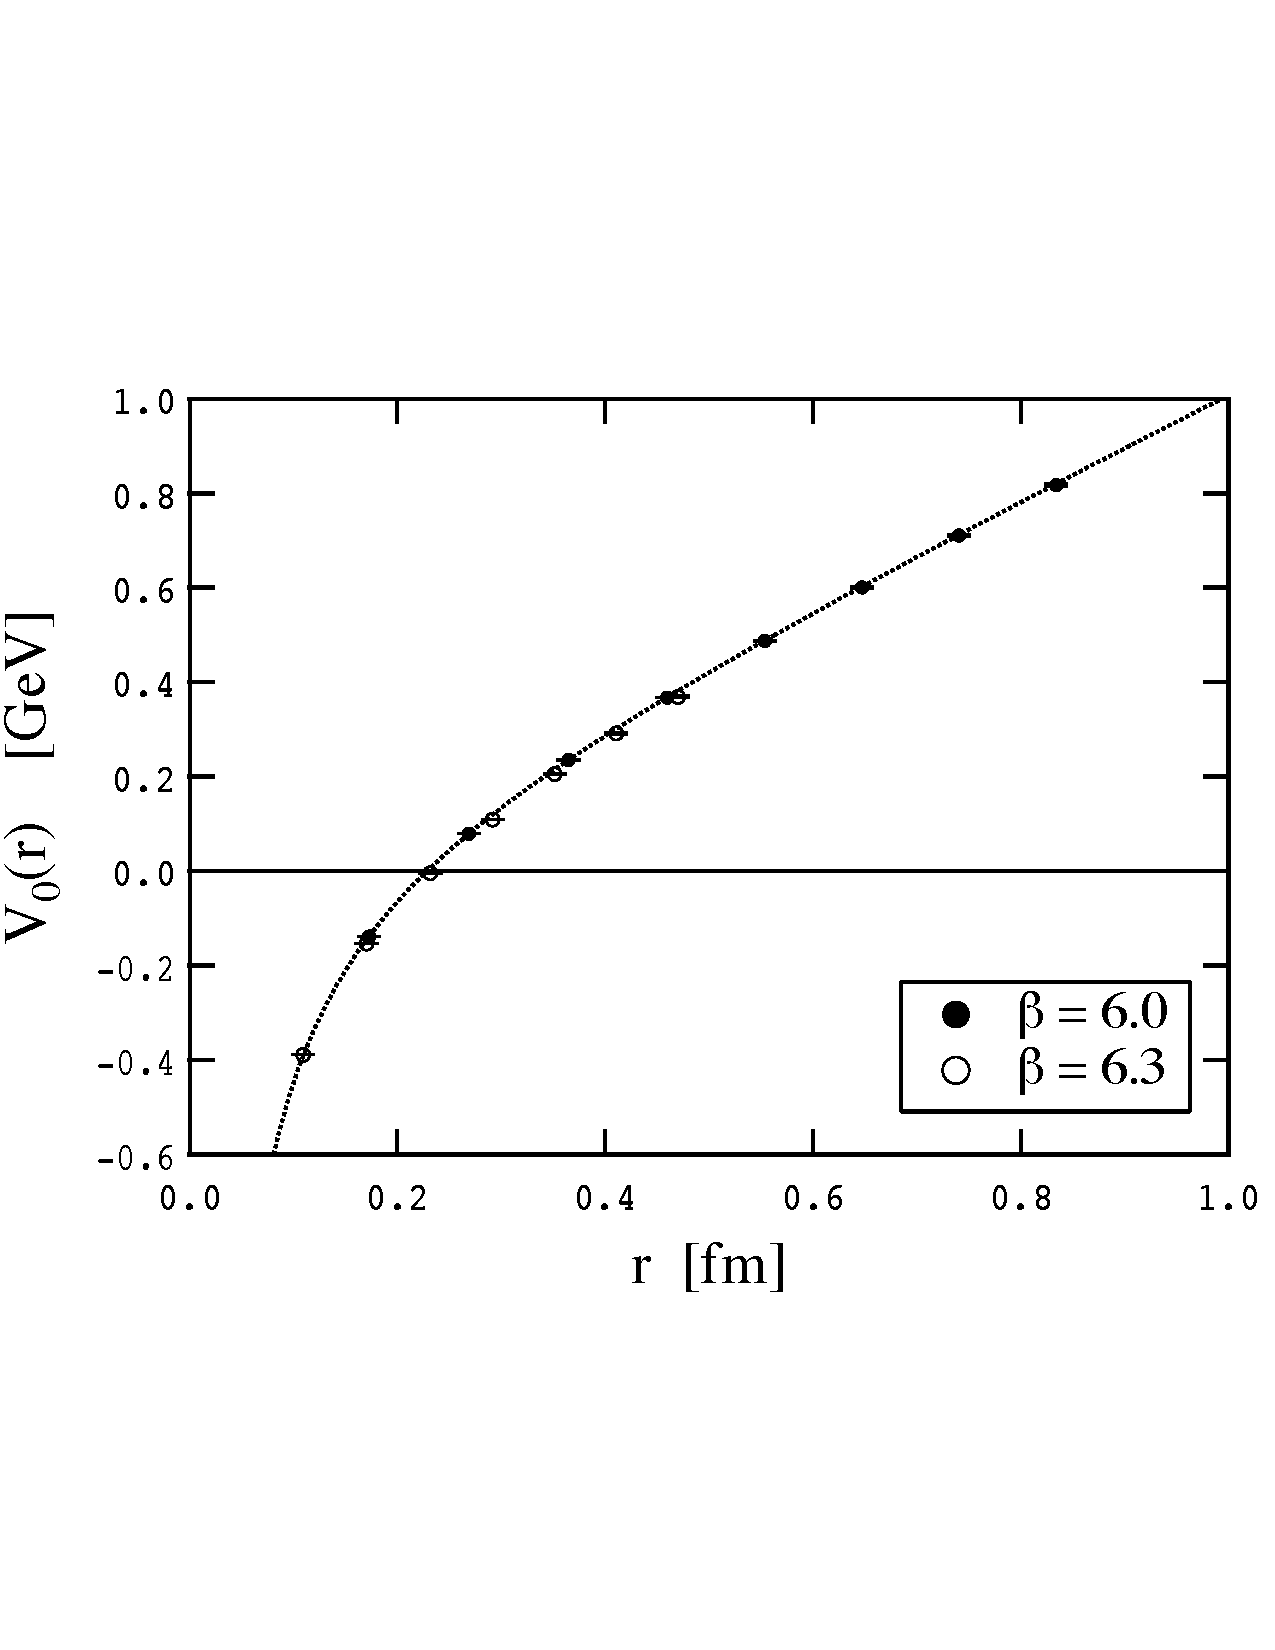
\includegraphics[width=0.4\textwidth]{figures/lattice_potential_qcd.pdf}
    \caption[Tracker material budget.]{
      The potential energy associated with two static quarks predicted by QCD as a function of distance, calculated numerically on the lattice.
      The potential increases roughly linearly with distance once a quark is no longer inside a hadron.
      The strong coupling used for the numerical calculation is denoted by $\beta$.
      Taken from \cite{lattice_potential}.}
    \label{fig:QCDpotential}
  \end{figure}  

  During a high energy collision involving a hadrons like a proton, quarks and gluons are customarily ejected, and eventually reach a great enough distance to trigger the formation of new hadrons.
  But, the ejection is oftentimes so violent that even this new hadron fragments, then these fragment, and so on.
  This produces a spray of hadrons and hadron decay products all traveling in approximately the same direction as the original ejected quark or gluon, a hadron jet.

  Unfortunately, the production of jets is difficult to predict experimentally due to yet another peculiar feature of QCD.
  The perturbative expansion described in the previous section is performed in powers of the interaction's coupling, with one factor of the coupling per vertex.
  In order for a truncated perturbation series to be a good approximation, the coupling must be significantly less than 1.
  Otherwise, diagrams with more vertices are in general more important than diagrams with fewer vertices, and no finite truncation can be accurate.
  Although the QCD coupling is less than 1 at high energy, making the perturbative approach still viable for very high energy collisions, the coupling explodes at low energies, which earns the strong interaction its name.

  \begin{figure}[h!]
    \centering
    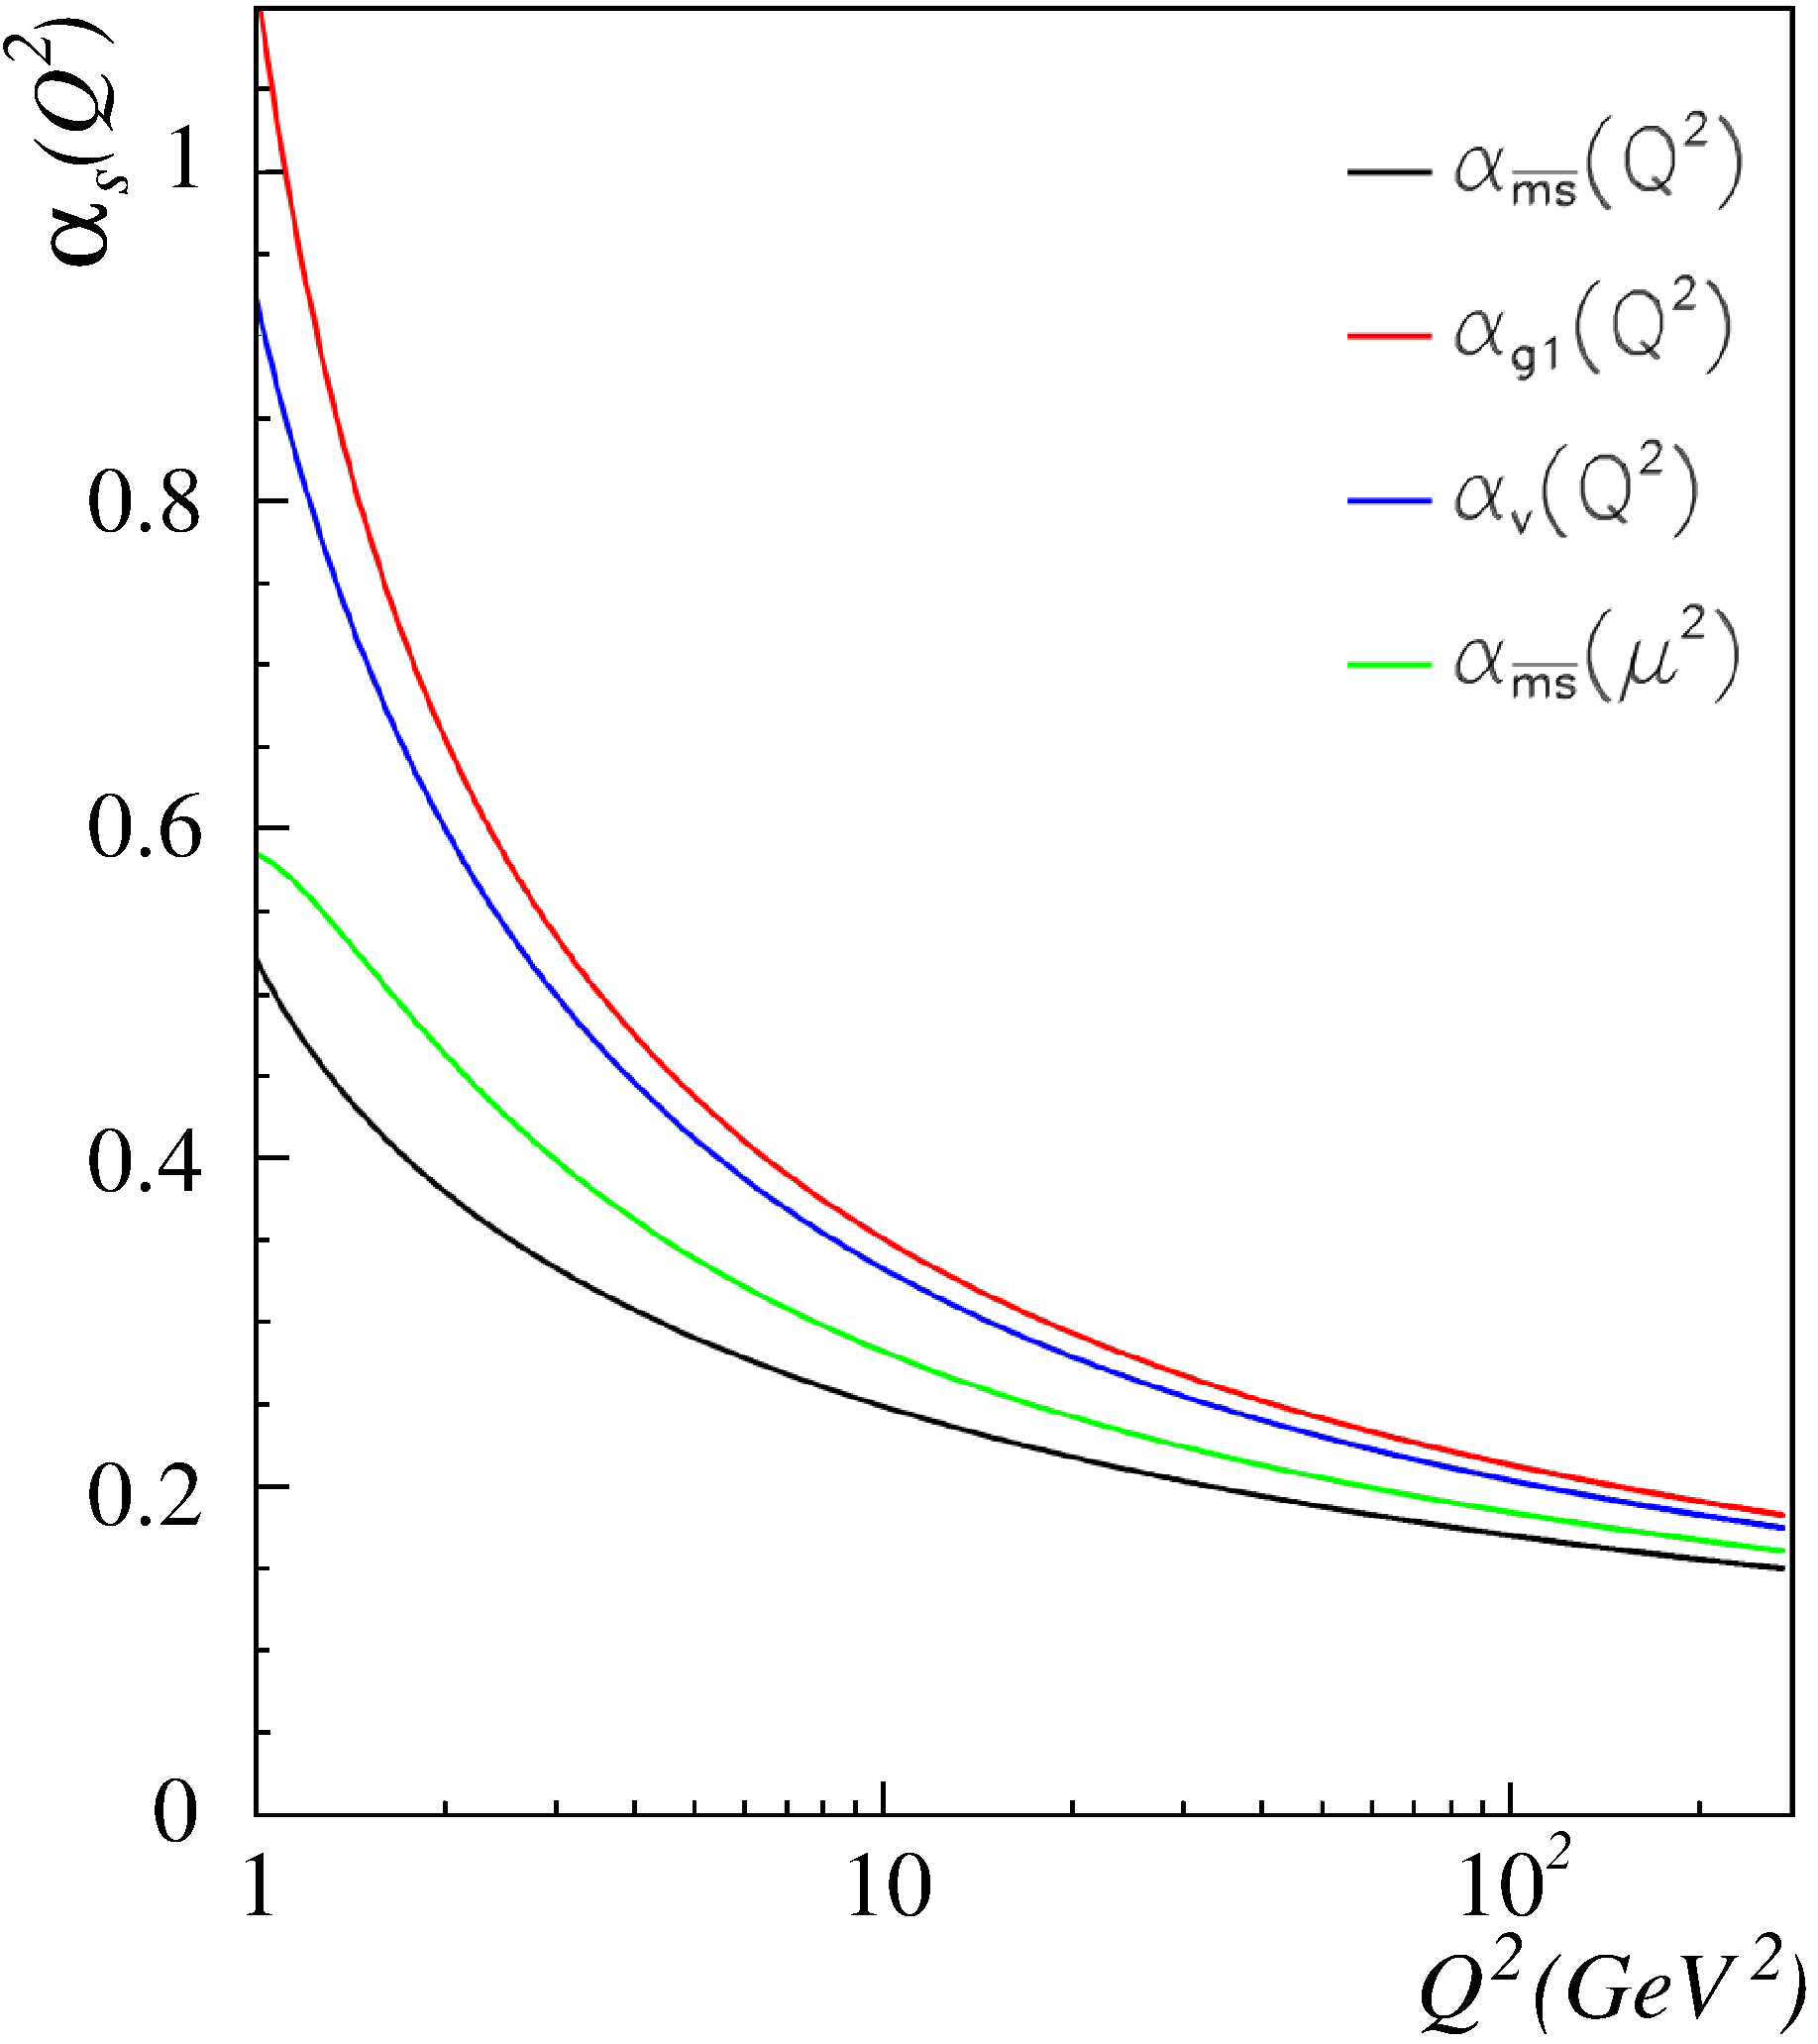
\includegraphics[width=0.4\textwidth]{figures/qcd_coupling.pdf}
    \caption[The QCD coupling as a function of the interaction energy.]{
      The QCD coupling explodes at low energy, making QCD non-perturbative for any interaction energy below around 1~GeV.
      The different lines are obtained for different methods of performing the calculation, specifically different renormalization schemes.
      Taken from \cite{qcd_coupling}.}
    \label{fig:QCDcoupling}
  \end{figure}  

  Non-perturbative approaches to QCD exist, including the lattice numerical method used to produce the plot shown in Figure~\ref{fig:QCDpotential}, but they are extremely computationally expensive for even the most simple calculations.
  It is not feasible to use make non-perturbative calculations of low energy QCD physics from first principles in an environment as complex as high energy hadron collisions.
  For the hadronization and fragmentation process, heuristic approximations tweaked to match data are used instead, typically the Lund String Model as implemented in the Pythia software package, see Section~\ref{sec:simulation}.
  Additionally, relatively low energy quarks and gluons can be emitted during the collision itself, called Initial State Radiation (ISR).
  A diagram of $u\bar{u} \rightarrow Z \rightarrow e^+e^-$ that includes a single ISR gluon is shown in Figure~\ref{fig:ISRdiag}.
  The most reliable way to predict ISR is to measure it in a very similar physics process, then convert this measurement to an expected rate in the physics process of interest.
  For example, ISR in $Z\rightarrow e^+e^-$ events is essentially identical to ISR in $Z\rightarrow \nu\nu$ events.
  
  \unitlength=2mm
  \begin{figure}[h!]
    \centering
    \begin{fmffile}{ISRdiag}
      \begin{fmfgraph*}(40,25)
        \fmfleft{i1,i2}
        \fmfright{o1,o2}
        \fmfbottom{b}
        \fmf{fermion,label=$u$,label.side=left}{i2,v1}
        \fmf{fermion,label=$\bar{u}$,label.side=left}{i1,vi}
        \fmf{fermion}{vi,v1}
        \fmf{gluon,label=ISR gluon,label.side=left}{vi,b}
        \fmf{photon,label=$Z$,label.side=left}{v1,v2}
        \fmf{fermion,label=$e^-$,label.side=left}{o2,v2}
        \fmf{fermion,label=$e^+$,label.side=left}{v2,o1}
      \end{fmfgraph*}
    \end{fmffile}

    \caption[A Feynamn diagram including an ISR gluon.]{
      Relatively low energy QCD can lead to the emission of Initial State Radiation as part of the hard collision, in this case $u\bar{u} \rightarrow Z \rightarrow e^+e^-$.
      This gluon will hadronize and add a jet to the event.
      ISR is difficult to predict accurately due to the intractability of QCD at low energy.
    }
    \label{fig:ISRdiag}
  \end{figure}  

  In summary, QCD's intractability at low energy combined with its raw strength make precise predictions of the outcome of hadron collisions difficult to obtain, despite the Standard Model's overall success in describing the interactions of elementary particles.
  The Standard Model prediction cannot always be obtained directly from first principles with satisfactory accuracy.

  \subsection{Parton Distribution Functions} \label{sec:PDFs}

  Being composite particles bound by QCD, the internal structure of hadrons is rich and difficult to understand quantitatively, due to the impossibility of using perturbation theory at the low energies that prevail in hadrons.
  The proton is often said to be a bound state of two up quarks and one down quark.
  This is true enough--the {\it net} composition of a proton is two up quarks and one down quark--but is an oversimplification.
  The quarks in a proton constantly emit and absorb gluons, which can split to quark-antiquark pairs, which can in turn annihilate back to gluons.
  Viewed at a small enough length scale, the proton is not a simple object, and not even a bound state of 3 quarks, but rather a complex cloud of quarks and gluons with various energies.
  This is problematic for any attempt to predict the outcome of proton collisions, because one cannot be sure which of these subcomponents, called partons, will be the componenent of the proton that actually experiences a collision.
  Due to the intractability of QCD at low energy, the composition of a proton is known only from a fit to data, and called a Parton Distribution Function (PDF).
  PDFs are typically expressed as the probability to find a parton of a given species carrying a given fraction of the proton's energy, as shown in Figure~\ref{fig:PDF}.
  These PDFs display a few sensible features described in the figure's caption.
  A large number of proton collisions samples all the possible initial partons, with momentum distributions described by the PDFs.
  Thus, a dataset composed of proton collisions naturally probes a wide range of energies.

  \begin{figure}[h!]
    \centering
    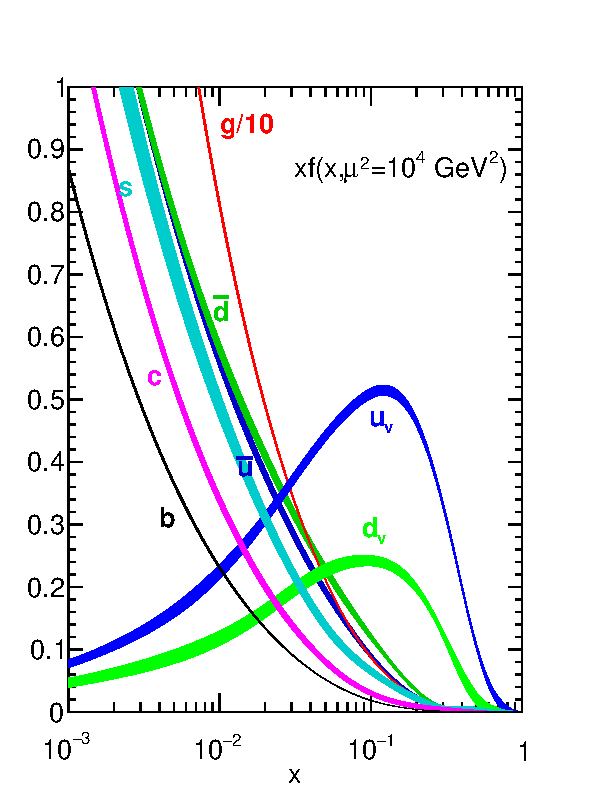
\includegraphics[width=0.4\textwidth]{figures/parton_distribution_function.pdf}
    \caption[Proton parton distribution function.]{
      The measured parton distribution function for a proton at an interaction energy of 100~GeV.
      The horizontal axis $x$ is the fraction of the proton's total momentum, and the vertical axis is the probability distribution.
      The finite thickness of the curves indicates the uncertainty.
      As one would expect for a proton, $uud$, the probability to collide with an up quark is around twice the probability to collide with a down quark at any energy.
      That $v$ subscript on these two curves indicate that these are the ``valence'' quarks, the only quarks that are present as more than transient products of gluon splitting.
      It is much less likely to find an up or down antiquark, and roughly equally likely to find either, because these antiquarks are produced only by gluon splitting.
      For the same reason, the probability to find a quark is exactly equal to the probability to find an antiquark for the heavier quark species, $s$, $c$, and $b$.
      Quarks aside, notice that the gluon curve (red) has been suppressed by a factor of 10 to fit on the plot.
      To a decent approximation, high energy proton collisions are in fact collisions between gluons.
      Taken from \cite{PDFs}.}
    \label{fig:PDF}
  \end{figure}  


\section{Some Problems with the Standard Model} \label{sec:SMproblems}

Standard Model is extremely successful (electron magnetic moment, Higgs prediction) but not entirely satisfactory.

  \subsection{Effective Field Theory} \label{sec:effective}

  Includes explicit energy cutoff, as part of renormalization.
  Cannot, by contruction, be the final theory.

  \subsection{Gravity} \label{sec:gravity}

  Doesn't include gravity, so Planck scale is maximum possible cutoff (but could be smaller).

  \subsection{The Hierarchy Problem} \label{sec:hierarchy}

  Why is the Higgs mass / weak scale so much smaller than the Planck scale?
  Is the cutoff much smaller?

  \subsection{Astrophysical Evidence of Dark Matter} \label{sec:DMevidence}

  SM has no (cold) dark matter candidate.
  Of course may be well out of reach, but look where we can.
  Good reason to believe that dark matter could be produced at LHC (WIMP miracle).

%  \subsection{The Strong CP Problem} \label{sec:strongCP}

\section{Supersymmetry} \label{sec:SUSY}

SUSY is one particular model that can patches up some of the SM's issues.

  \subsection{Theoretical Appeal} \label{sec:SUSYappeal}

  Solves up hierarchy problem if at the weak scale (so, potentially accessible to LHC) and provides a dark matter candidate.
  (Focus on RPC SUSY, due to proton stability.)

  \subsection{Experimental Signatures} \label{sec:SUSYexp}

  SUSY produces MET, and in strong SUSY decays, potentially lots and lots of jets.
  Since SUSY

  \subsection{Simplified Models} \label{sec:SUSYsms}

  SUSY parameter space is vast, so we consider one potential discovery channel at a time.

  \begin{figure}[h!]
    \centering
    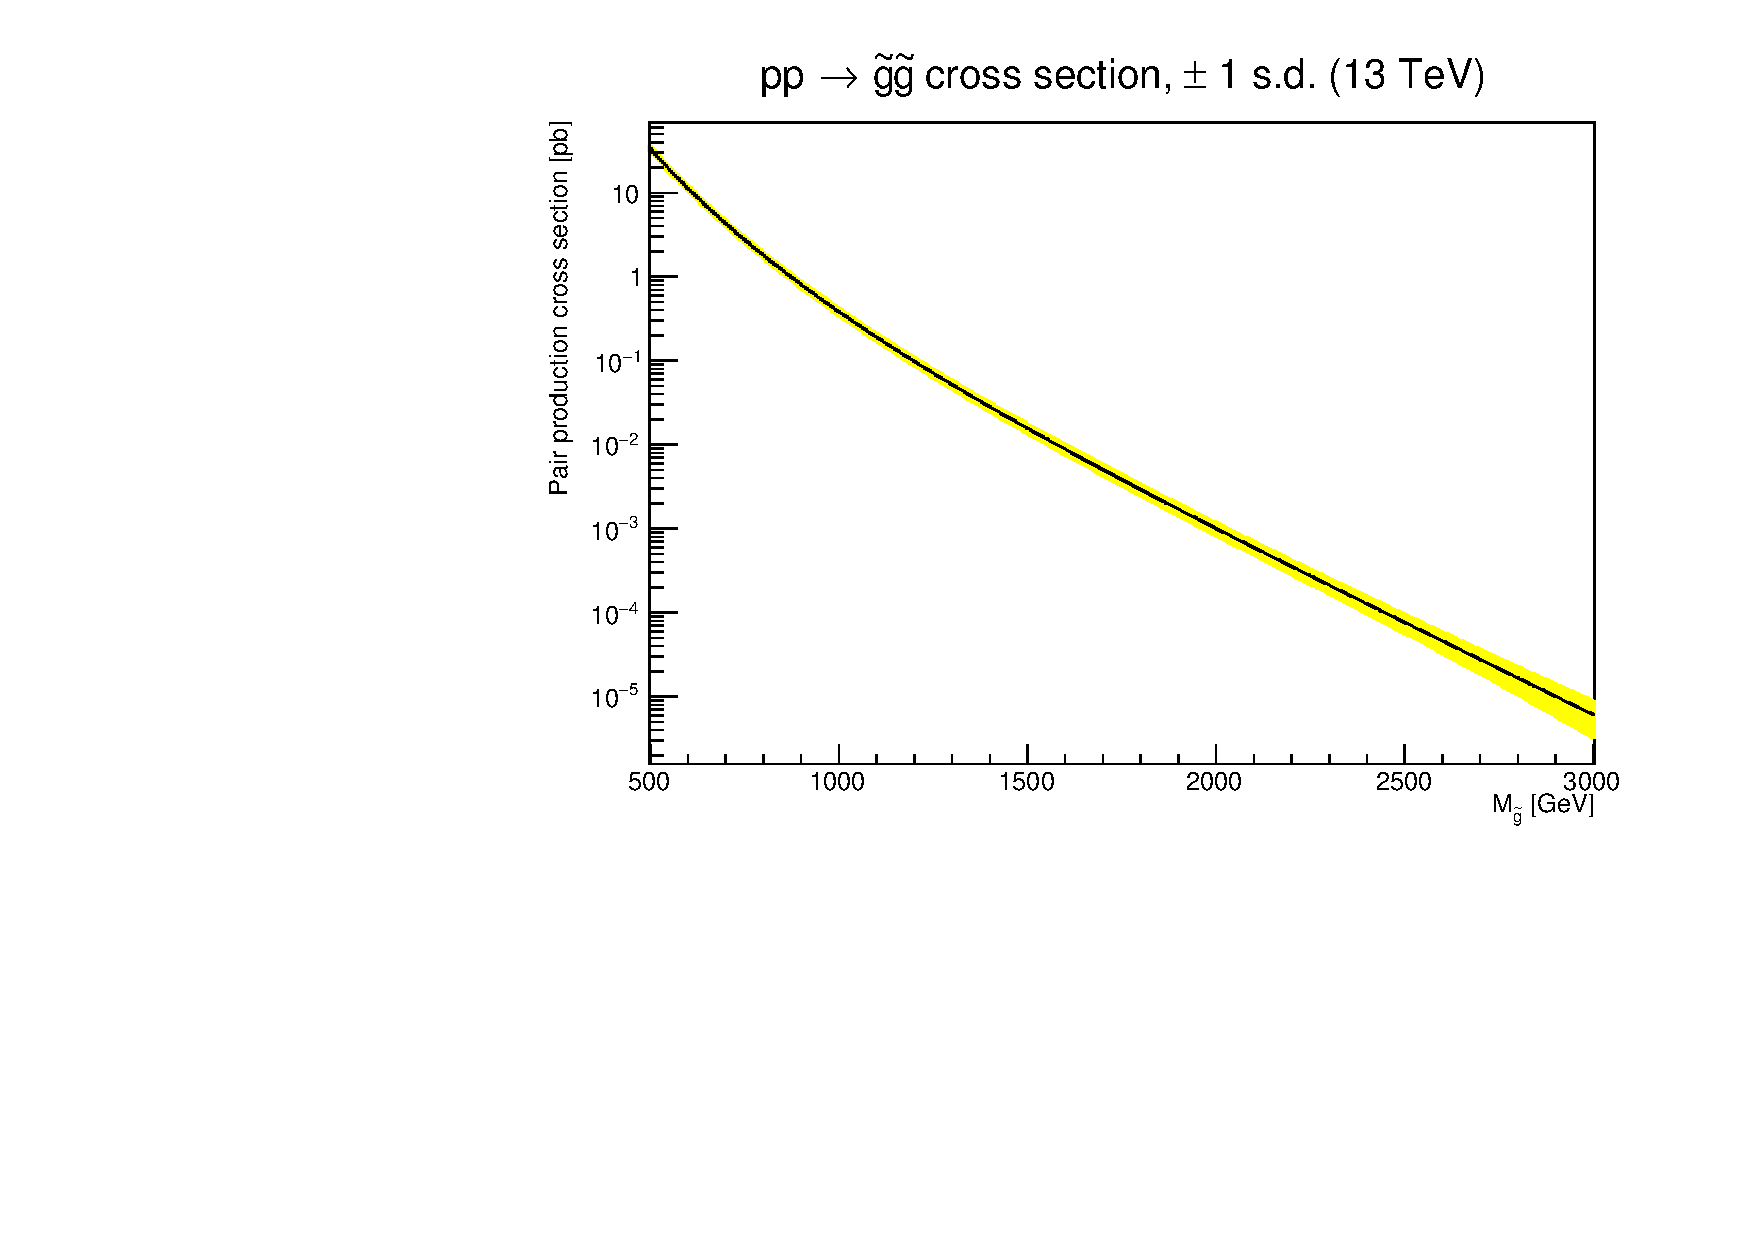
\includegraphics[width=0.85\textwidth]{figures/gluino_xsec.pdf}
    \caption[Theoretical gluino pair production cross section in simplified models.]{In simplified models, it is possible to calculate superpartner production cross sections from theory.
Here, the theoretical gluino pair production cross section in 13 TeV proton-proton collisions is shown in black, with the one standard deviation uncertainty shown as a yellow band.
The cross section drops rapidly with increasing mass.
Based on cross section values used in \cite{MT2_2019}, calculated in \cite{SUSYxsecs}.
Compare Figure 5 (upper) from \cite{SUSYxsecs}, of which this is a simplified reproduction.
}
    \label{fig:SUSYxsec}
  \end{figure}  

\section{Other Models} \label{sec:othermodels}

Introduce leptoquarks and mono-$phi$.

